\chapter{Background}
\label{BG}
\section{Problem area}
\label{BG-PR}
% Web-maps -> Maps on the web / digital maps / maps on the computer?
% A negative side-effect of the web maps, is that it isn't as easy to bring 
% along on a trip, as a traditional road map.
Over the last decade people have switched from traditional roadmaps 
to using the web-maps. This is a change without any significant negative side-effects. 
The online services remove all the problems with determining the quickest 
route between two points and you spend no time flipping the pages of 
the map to find what you need. With the smartphones on the market today, 
the online maps are even more useful, since you no longer need to 
prepare your trip before you leave.

The online maps have now been used for many years and haven`t been slow 
at adopting new features to improve their usability. Many has 
implemented satellite-maps, that allow us to see the entire planet 
from above, and lately the feature called Google Street View has upped 
the stakes, when allowing us to look in any direction from a given point 
of a road. The two maps that we use the most are Google Maps and the 
Danish map called Krak. These maps both have the mentioned features 
but slight differences in the way the user navigates and searches 
for routes.

Because of the widespread knowledge of the online maps, the users 
have grown accustomed to certain features and ways of using the map. 
It is very important that we, with a new map program, use this knowledge 
to our advantage and don`t try to reinvent the wheel. By using some 
of the commonly used controls in our map, a user will be able to quickly 
adapt to our program and use it efficiently. 

\section{Requirements for the map}
\label{BG-R}
Our teachers had a few requirements for features in the project. The
requirements were presented to us during development, in 3 steps. This made it
easier for us to focus on getting the basic features of the program to work, but
it made it harder for us to plan ahead as well.

Here is a list of the features we had to implement: 
\begin{itemize}
  \item We had to make a visual representation of all the roads from the
  dataset.
  \item We had to draw different kinds of roads in different colors.
  \item We had to adjust our drawing of the roads, to the window size of our
  user interface.
  \item We had to make mouse zooming possible.  The user should be able to drag
  and select an area with the mouse, creating a square or rectangle, and zoom in on the
  selected area.
  % It isn't important whether or not it is a method. Should be slightly re-phrased.
  \item We had to implement a method to find a route from one point on the map to
  another, and we had to allow the user to find that route by clicking at each
  of the points.
\end{itemize}
% ``Of course, some of the...'' sounds a bit cocky for my taste.
% Should probably be re-phrased a bit.
We had to consider these requirements while
deciding how the program should be designed. Of course, some of the
requirements were so self explanatory that we would have made them regardless
of them being required.

\section{Our requirements}
In the process of designing the program, we made some requirements, that we
wanted to make sure was met, before making more advanced features. Since it was
required to make the user able to zoom-in on the map, we found it logical to
allow him or her to:
\begin{itemize}
  \item Zoom out
  \item Pan around on the map
\end{itemize}

With these basic features covered, we decided which advanced featured we wanted
to implement. In order to give the user a chance to find more specific places, we
decided to show the user the name of the road closest to the cursor. This means
that the user can get orientated without clicking or pressing any buttons. 

% Why is it due to the size of the maps, that there isn't a way of selecting bike-tours?
% The length of the edges are present, which is the only thing needed, right?
The most interesting feature of our \class{Map of Denmark} is perhaps the
option of selecting whether you want to travel by car or by bicycle. Many Danish
people use bicycles to travel and as such this feature is a very relevant and
nice one to have in the software. It is a feature not usually seen on
international maps - this is most likely due to the size of these maps.

% ``This makes our map well suited...'' sounds a bit too confident.
We also decided to let the user create routes with an unlimited amount of
waypoints. This makes our map well suited for planning bicycling trips or longer
car rides where you want to reach more than one destination. Because this
feature can be quite demanding when a lot of waypoints are selected, we had to
make sure that the algorithm for finding routes was fast enough to ensure that the 
map is pleasant to use.

We wanted to make sure that the shape of Denmark is recognizable when
the user is zoomed far enough out to show the entire country. There is a balance between
showing a big amount of roads and the delay when navigating. We wanted to make
the user able to navigate the map with an acceptable delay. 

The fact that we chose specific requirements for our program gave us two big
advantages. It both made the planning process easier, and it did the design phase a lot 
easier, when we knew what the program should be able to do. In the process of creating the
program, we had to change and create new requirements for ourselves, when we
felt some feature was necessary for the end-user to have. In the last part of
the coding process, we decided on our final requirements and worked towards completing them. 

\section{Data set}
\label{BG-DS}
% This could be longer.
We have been provided with a dataset of roads and intersections in Denmark 
from Krak. Additionally we were given some code for loading the data from the 
text files.

\subsection{UTM-coordinates}
\label{BG-DS-UTM}
% What is KrakNode? What is UTM32? How is it important?
When using the UTM standard the earth is divided into 60 rectangles that each 
has the origo at the south-west corner. Most of Denmark is within the UTM-32 
rectangle so all the coordinate data is given as UTM32-coordinates.
These coordinates need some conversion when used in Java since the origo is placed 
differently. This will be explained further in the section about \nameref{UTM-conversion}
on page \pageref{UTM-conversion}.

\subsection{Graph}
\label{BG-DS-G}
When the data has been loaded it is stored as a \class{Graph} object containing 
\class{KrakNode}s and \class{KrakEdge}s. The \class{KrakEdge}s are the 
road segments and contains the name of the road, an estimated drive time, 
a direction of traffic and references to the two \class{KrakNode}s that are at 
either end of the road.  The \class{KrakNode} itself contains only the coordinates 
for the point. The \class{Graph} contains a number of useful methods for 
searching the data like getting all edges that is connected to a \class{KrakNode}. 
We will be using these methods extensively throughout the project both for 
drawing the map and for finding the route between two points.
% ^ False - we use the quadtree for drawing the map, right?
% ``Extensively'' should probably be re-phrased. It indicates ``a lot'', and it isn't 
% that much and that important, that the user knows that.

\section{MVC structure}
\label{BG-MVC}
In order to achieve a decent code structure and separation of responsibilities, 
we utilize the Model-View-Controller (MVC) architecture. By doing this, we split 
the code into smaller sections, which can be easier to handle and easier to 
coorporate on the code.

This is because we split the code into three parts: graphical user interface 
(``view''), data handling (``model'') and the connection between the two 
(``controller''). Read more in section \ref{UML} \class{\nameref{UML}} on 
page \pageref{UML}.

\subsection{What is it? How does it work?}
In order to achieve a decent code structure, it is important to split the 
responsibilities of the program into different pieces, which work together 
to make the program work as intended.

One way to do this, is to have the graphical user interface in a class of its
own, and the rest of the program in another class. The downside to this
approach, is that it can get ambiguously where to put specific pieces of code
(button listeners and such).

We chose to utilize the Model-View-Controller (MVC) architecture, which is
another way of structuring a program (a better one). With MVC we divide our code
in three main parts, in order to achieve a decent separation of data, logic and
the graphical interface.

\begin{figure}[h!]
\centering
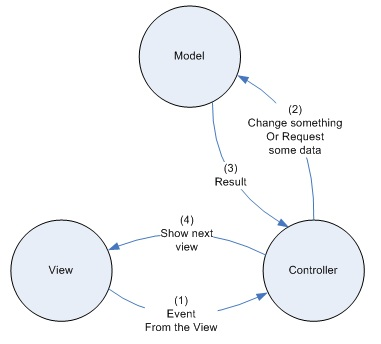
\includegraphics[width=0.5\linewidth]{images/mvc}
\caption{Overview of MVC}
\label{mvc-overview}
\end{figure}

Like the picture above shows, every graphical window has its own class. These
classes are called ``views''. Where we beforehand had one class to handle both
communication with the data and the graphical windows, we now split this into
two: ``models'' and ``controllers''.

The models handle all communication with the data sources, and every model
handle one data source. If we were to use relational databases, we would have a
model for each table in the database. In our case we only have one data source
(Krak's dataset), and therefore only have one model, to communicate with this.

Controllers
Now we only need a way to connect the graphical interface with the data. This is
where controllers enter the picture. In MVC you have one controller per view.
This controller provides the view with all the neccessary data from the models.
The controllers also have listeners on the view, that listens to events on the
view (like when the user presses a button, clicks his/her mouse and such). Then
the controller can provide new data to the view or save new data from the view
to the data source (through the models).

An example of this could be that the user updates some info and presses the 
``Save''-button. Then the controller listens to this event, passes the new data
to the models and it gets saved.
In our case we have listeners to (among other things) mouseclicks, so we can
place pins when the user clicks the map.